\documentclass{article}
\usepackage{tikz}
\usetikzlibrary{positioning}
\begin{document}

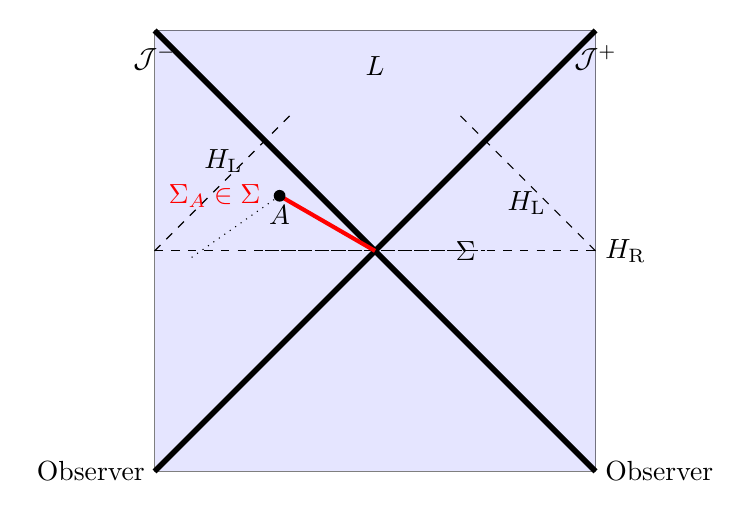
\begin{tikzpicture}[scale=0.7]
    % Draw the square representing the spacetime diagram
    \draw[fill=blue!20,opacity=0.5] (-4,-4) -- (4,-4) -- (4,4) -- (-4,4) -- cycle;
    
    % Label the regions
    \node at (4,3.5) {$\mathcal{J}^+$};
    \node at (-4,3.5) {$\mathcal{J}^-$};
    
    % Draw the horizons H_L and H_R
    \draw[dashed] (-4,0) -- (4,0) node[right] {$H_{\rm R}$};
    \draw[dashed] (-4,0) -- (-1.5,2.5) node[midway,above] {$H_{\rm L}$};
    \draw[dashed] (4,0) -- (1.5,2.5) node[midway,below] {$H_{\rm L}$};
    
    % Draw the observers
    \node[left] at (-4,-4) {Observer};
    \node[right] at (4,-4) {Observer};
    
    % Draw the diagonal lines forming the cosmological horizons
    \draw[line width=2pt] (-4,-4) -- (4,4);
    \draw[line width=2pt] (-4,4) -- (4,-4);
    
    % Draw the dashed line and the sphere A
    \draw[dashed] (-2,0) -- (0,0) -- (2,0) node[left] {$\Sigma$};
    \draw[line width=1.5pt,red] (0,0) -- ++(150:2) node[black,circle,fill=black,inner sep=1.5pt,label={[red]left:$\Sigma_A\in\Sigma$}] (A) {};
    \draw[dotted] (A.center) -- ++(35:-2); % Future lightsheet
    
    % Label points A and L
    \node at (A) [below] {$A$};
    \node at (0,3) [above] {$L$};
\end{tikzpicture}

\end{document}